% !TEX root = ../main.tex

\appendix

\section{Code snippets} \label{app:code-snippets}

\begin{lstlisting}
private void generateTree(Vertex vertex, int leftIndex, int rightIndex) {

    vertex.leftKey = leftIndex;
    vertex.rightKey = rightIndex;

    if (!vertex.isLeaf()) {

        int separatorIndex = (leftIndex + rightIndex) / 2;

        Vertex leftChild = new Vertex();
        vertex.left = leftChild;
        generateTree(leftChild, leftIndex, separatorIndex);

        Vertex rightChild = new Vertex();;
        vertex.right = rightChild;
        generateTree(rightChild, separatorIndex + 1, rightIndex);

        // Min and max is calculated from the children
        vertex.minMax = MinMax.combine(leftChild.minMax, rightChild.minMax);

    } else {

        // The vertex is a leaf, so leftIndex = rightIndex
        double value = values[leftIndex];
        vertex.minMax = new MinMax(value, value);

    }
}
\end{lstlisting}

\begin{lstlisting}
public MinMax getMinMax(int leftKey, int rightKey) throws Exception {
    return getMinAndMaxHelper(leftKey, rightKey, root);
}

private MinMax getMinAndMaxHelper(int a, int b, Vertex x) throws Exception {

    if (x.isLeaf())
        return x.minMax;

    // The two paths are following each other, ie. this node is on both paths.
    if (x.left.inInterval(a) && x.left.inInterval(b)) {
        return getMinAndMaxHelper(a, b, x.left);
    } else if (x.right.inInterval(a) && x.right.inInterval(b)) {
        return getMinAndMaxHelper(a, b, x.right);
    }

    // The two paths are splitting up AT THIS NODE
    if (x.left.inInterval(a) && x.right.inInterval(b)) {
        return MinMax.combine(getMinAndMaxHelper(a, b, x.left),
                                getMinAndMaxHelper(a, b, x.right));
    }

    // The two paths have already split apart. This means that the current
    // node is only on the path to ONE of the two endpoints, either the left
    // path or the right path.
    if (x.left.inInterval(a)) {
        return MinMax.combine(getMinAndMaxHelper(a, b, x.left), x.right.minMax);
    } else if (x.right.inInterval(a)) {
        return getMinAndMaxHelper(a, b, x.right);
    }

    if (x.right.inInterval(b)) {
        return MinMax.combine(getMinAndMaxHelper(a, b, x.right), x.left.minMax);
    } else if (x.left.inInterval(b)) {
        return getMinAndMaxHelper(a, b, x.left);
    }

    // If this is reached then the interval is not valid
    throw new Exception("The interval is not valid");
}
\end{lstlisting}

\section{Class diagrams} \label{app:class-diagrams}


\begin{figure}[ht]
    \centering
    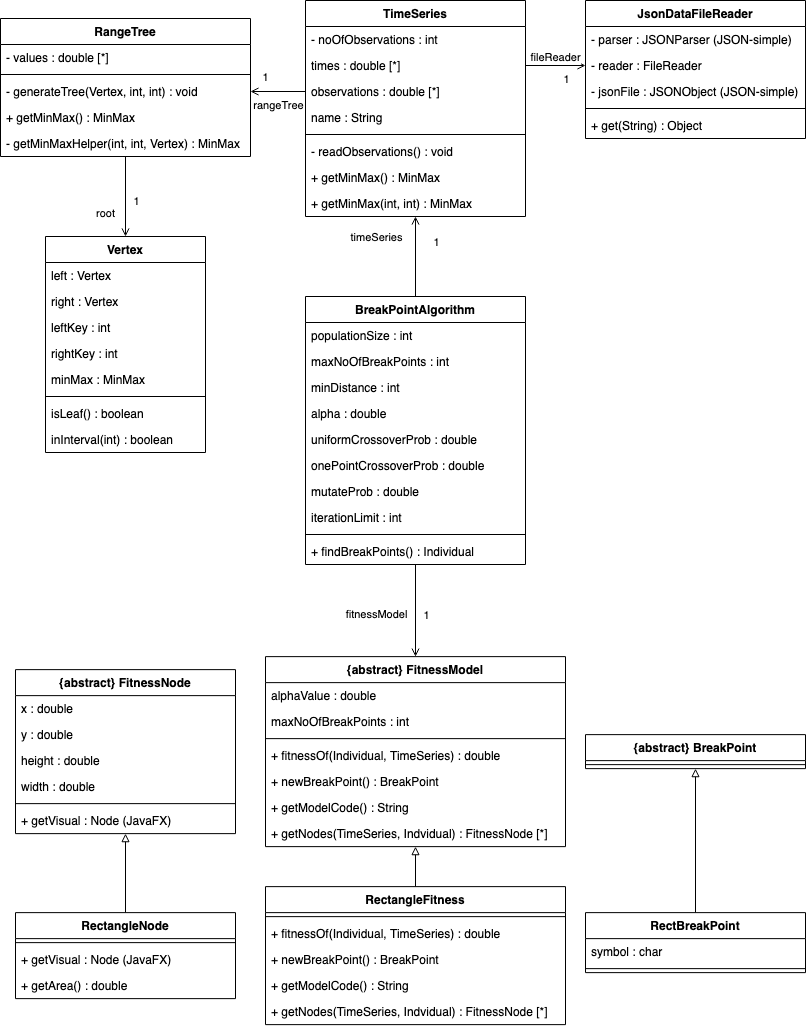
\includegraphics[width=.8\textwidth]{fig/class-diagram-algorithm.png}
    \caption{Class diagram of the break point algorithm with time series and fitness}
    \label{fig:class-diagram-algorithm}
\end{figure}